\documentclass{article}
\usepackage{graphicx}
\usepackage{amsmath}

\begin{document}
\title{Maths Assignment}
\author{Karyampudi Meghana Sai\\ EE23BTECH11031}
\maketitle

\section*{Problem Statement}
Write the first five terms of the sequence \(a_n = \frac{n(n^2+5)}{4}\).

\section*{Solution}
The sequence x(n):
\begin{align}
x(n) &= \frac{(n+1)((n+1)^2+5)}{4}\\
x(n)&=\frac{(n+1)^3+5(n+1)}{4}\\
x(n)&=\frac{n^3+3n^2+8n+6}{4}
\end{align}
 





The relation between x(n) and u(n):
\begin{align}
 x(n) = \left(\frac{(n+1)^3+5(n+1)}{4}\right) \cdot u(n)
 \end{align}
Finding the z transform of u(n):
\begin{align}
U(z) = \mathcal{Z}\{u(n)\} = \sum_{n=0}^{\infty} u(n)z^{-n}
\end{align}

Given that the unit step function \(u(n)\) is:

\begin{align} 
u(n) = \begin{cases} 0 & \text{if } n < 0 \\ 1 & \text{if } n \geq 0 \end{cases}
 \end{align}

Its Z-transform becomes:

\begin{align}
U(z) &= \sum_{n=0}^{\infty} z^{-n} = 1 + z^{-1} + z^{-2} + z^{-3} + \dotsb  \\
U(z) &= \frac{1}{1- z^{-1}}
\end{align}
ROC for the z transform of u(n):\\
\text{ROC for } U(z):$\lvert z \rvert > 1$



The $z$ transform of $nu(n)$ can be derived as follows:

Given the signal $nu(n)$, its $z$ transform is represented as:

\begin{align}
\mathcal{Z}\{nu(n)\} = \sum_{n=0}^{\infty} nu(n)z^{-n}
\end{align}

The signal $nu(n)$ means the product of $n$ and the unit step function $u(n)$:

\begin{align}
nu(n) = n \cdot u(n)
\end{align}

The $z$ transform of $u(n)$ is $U(z) = \frac{z}{z-1}$. To find the $z$ transform of $nu(n)$, let's derive it step by step:

\begin{align}
\mathcal{Z}\{nu(n)\} &= \sum_{n=0}^{\infty} nu(n)z^{-n} \\
\mathcal{Z}\{nu(n)\}&= \sum_{n=0}^{\infty} n \cdot u(n)z^{-n}
\end{align}

Now, this expression involves the convolution property of the $z$ transform. The $z$ transform of $n$ is derived separately as:

\begin{align}
\mathcal{Z}\{n\} = \sum_{n=0}^{\infty} nz^{-n-1} = \frac{z^{-1}}{(1-z^{-1})^2}
\end{align}

By convolving the $z$ transform of $n$ with $U(z)$, we get:

\begin{align}
\mathcal{Z}\{nu(n)\} = U(z) * \mathcal{Z}\{n\}
\end{align}

Therefore, after convolution:

\begin{align}
\mathcal{Z}\{nu(n)\} = U(z) \cdot \mathcal{Z}\{n\} = \frac{1}{1-z^{-1}} \cdot \frac{z^{-1}}{(1-z^{-1})^2}
\end{align}

Simplifying the expression:

\begin{align}
\mathcal{Z}\{nu(n)\} = \frac{z^{-1}}{(1-z^{-1})^3}
\end{align}

The $z$ transform 0f $n^2u(n)$ can be derived as follows:

\begin{align}
\mathcal{Z}\{n^2u(n)\} = \sum_{n=0}^{\infty} n^2u(n)z^{-n} \end{align}

Now, $n^2$ can be represented as a signal $n^2$ convolved with the unit step function $u(n)$:

\begin{align}
 n^2u(n) = n^2 * u(n) 
 \end{align}

Using the property that $\mathcal{Z}\{f(n) * g(n)\} = F(z)G(z)$:

\begin{align}
 \mathcal{Z}\{n^2 * u(n)\} = \mathcal{Z}\{n^2\} \cdot \mathcal{Z}\{u(n)\}
  \end{align}

The $z$ transform of $n^2$ is found to be:

\begin{align}
 \mathcal{Z}\{n^2\} = \sum_{n=0}^{\infty} n^2z^{-n-1} = \frac{(z^{-1})(1+z^{-1})}{(1-z^{-1})^3}
  \end{align}



Therefore, the $z$ transform of $n^2u(n)$ can be obtained by multiplying the $z$ transforms of $n^2$ and $u(n)$:

\begin{align}
\mathcal{Z}\{n^2u(n)\} &= \mathcal{Z}\{n^2\} \cdot \mathcal{Z}\{u(n)\} \\
\mathcal{Z}\{n^2u(n)\}&= \frac{(z^{-1})(1+z^{-1})}{(1-z^{-1})^3} \frac{1}{1-z^{-1}} \\
\mathcal{Z}\{n^2u(n)\}&= \frac{(z^{-1})(1+z^{-1})}{(1-z^{-1})^4} 
\end{align}


The $z$ transform 0f $n^3u(n)$ can be derived as follows:

\begin{align}
\mathcal{Z}\{n^3u(n)\} = \sum_{n=0}^{\infty} n^3u(n)z^{-n} \end{align}

Now, $n^3$ can be represented as a signal $n^3$ convolved with the unit step function $u(n)$:

\begin{align}
 n^3u(n) = n^3 * u(n) 
 \end{align}

Using the property that $\mathcal{Z}\{f(n) * g(n)\} = F(z)G(z)$:

\begin{align}
 \mathcal{Z}\{n^3 * u(n)\} = \mathcal{Z}\{n^3\} \cdot \mathcal{Z}\{u(n)\}
  \end{align}

The $z$ transform of $n^3$ is found to be:

\begin{align}
 \mathcal{Z}\{n^3\} = \sum_{n=0}^{\infty} n^3z^{-n-1} = \frac{(z^{-1})(1+z^{-1})(1+2z^{-1})}{(1-z^{-1})^4}
  \end{align}



Therefore, the $z$ transform of $n^3u(n)$ can be obtained by multiplying the $z$ transforms of $n^3$ and $u(n)$:

\begin{align}
\mathcal{Z}\{n^3u(n)\} &= \mathcal{Z}\{n^3\} \cdot \mathcal{Z}\{u(n)\} \\
\mathcal{Z}\{n^3u(n)\}&= \frac{(z^{-1})(1+z^{-1})(1+2z^{-1})}{(1-z^{-1})^4} \frac{1}{1-z^{-1}} \\
\mathcal{Z}\{n^3u(n)\}&= \frac{(z^{-1})(1+z^{-1})(1+2z^{-1})}{(1-z^{-1})^5} 
\end{align}

Z-Transform of x(n):
\begin{align}
X(z) &=  \frac{\mathcal{Z}\{n^3u(n)\}}{4}+ \frac{\mathcal{Z}\{3n^2u(n)\}}{4}+ \frac{\mathcal{Z}\{8nu(n)\}}{4}+ \frac{\mathcal{Z}\{6u(n)\}}{4}\\
X(z)&= \frac{(z^{-1})(1+z^{-1})(1+2z^{-1})}{4(1-z^{-1})^5}+ \frac{3(z^{-1})(1+z^{-1})}{4(1-z^{-1})^4}+\frac{8z^{-1}}{4(1-z^{-1})^3}+\frac{6}{4(1- z^{-1})}
\end{align}
\newpage
Here's the plot of x(n):

\begin{figure}[h]
  \centering
  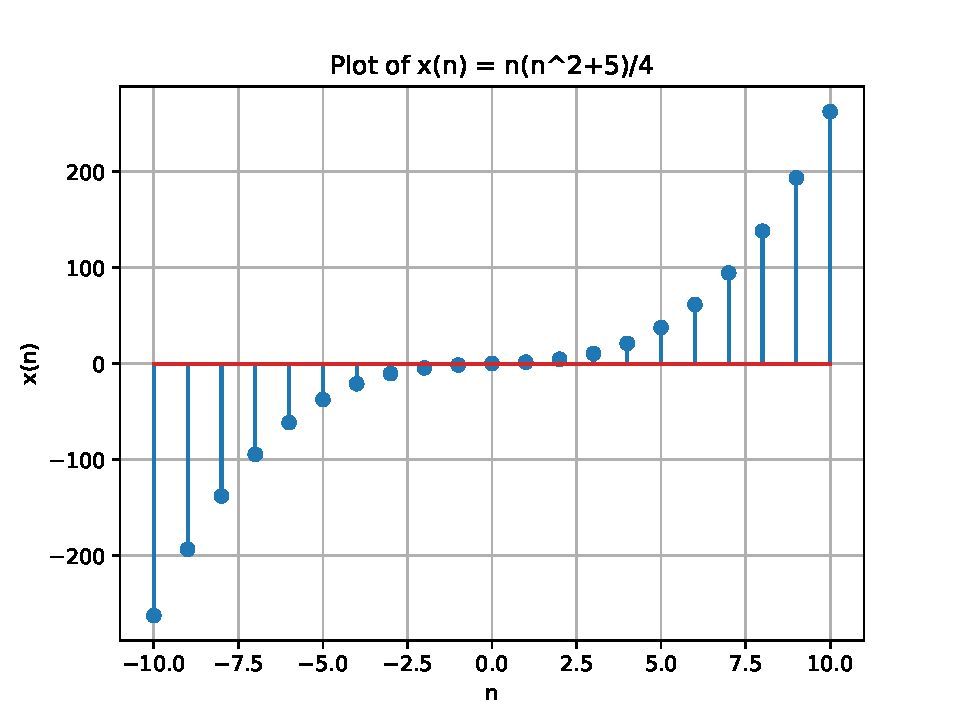
\includegraphics[width=0.8\textwidth]{plot.pdf} % Adjust width if needed
  \caption{Plot of the function $x(n) = \frac{(n+1)((n+1)^2+5)}{4}$}
  \label{fig:plot}
\end{figure}


\end{document}

